\documentclass[12pt]{article}
\usepackage{fullpage}
\usepackage{hyperref}
\hypersetup{bookmarks=true,colorlinks=true,linkcolor=red,citecolor=blue,filecolor=magenta,urlcolor=cyan}
\usepackage{amsmath}
\usepackage{longtable}
\usepackage{booktabs}
\usepackage{caption}
\usepackage{graphics}
\title{Software Requirements Specification for Solar Water Heating Systems}
\author{Thulasi Jegatheesan}
\begin{document}
\maketitle
\tableofcontents
\newpage
\section{Reference Material}
\label{Sec:RM}
This section records information for easy reference.
\subsection{Table of Units}
\label{Sec:ToU}
The unit system used throughout is SI (Syst\`{e}me International d'Unit\'{e}s). In addition to the basic units, several derived units are also used. For each unit, the table lists the symbol, a description and the SI name.
\begin{longtable*}{l l}
\toprule
Symbol & Description
\\
\midrule
m & length (metre)
\\
kg & mass (kilogram)
\\
s & time (second)
\\
${}^{\circ}C$ & temperature (centigrade)
\\
J & energy (joule)
\\
W & power (watt)
\\
\bottomrule
\label{Table:ToU}
\end{longtable*}
\subsection{Table of Symbols}
\label{Sec:ToS}
The table that follows summarizes the symbols used in this document along with their units. The choice of symbols was made to be consistent with the heat transfer literature and with existing documentation for solar water heating systems. The symbols are listed in alphabetical order.
\begin{longtable*}{l l 1}
\toprule
Symbol & Description & Units
\\
\midrule
$A_{C}$ & $\text{m}^{2}$ & Coil surface area
\\
$A_{in}$ & $\text{m}^{2}$ & Surface area over which heat is transferred in
\\
$A_{out}$ & $\text{m}^{2}$ & Surface area over which heat is transferred out
\\
$C$ & $\frac{\text{J}}{(\text{kg}{}^{\circ}C)}$ & Specific heat capacity
\\
$C^{L}$ & $\frac{\text{J}}{(\text{kg}{}^{\circ}C)}$ & Specific heat capacity of a liquid
\\
$C_{W}$ & $\frac{\text{J}}{(\text{kg}{}^{\circ}C)}$ & Specific heat capacity of water
\\
$D$ & m & Diameter of tank
\\
$g$ & $\frac{\text{W}}{\text{m}^{2}}$ & Volumetric heat generation per unit volume
\\
$h$ & $\frac{\text{W}}{(\text{m}^{2}{}^{\circ}C)}$ & Convective heat transfer coefficient
\\
$h_{C}$ & $\frac{\text{W}}{(\text{m}^{2}{}^{\circ}C)}$ & Convective heat transfer between coil and water
\\
$L$ & m & Length of tank
\\
$m$ & kg & Mass
\\
$m_{W}$ & kg & Mass of water
\\
$q$ & $\frac{\text{W}}{(\text{m}^{2}{}^{\circ}C)}$ & Heat flux
\\
$\mathbf{q}$ & $\frac{\text{W}}{\text{m}^{2}}$ & Thermal flux vector
\\
$q_{C}$ & $\frac{\text{W}}{\text{m}^{2}}$ & Heat flux from coil
\\
$q_{in}$ & $\frac{\text{W}}{\text{m}^{2}}$ & Heat flux in
\\
$q_{out}$ & $\frac{\text{W}}{\text{m}^{2}}$ & Heat flux out
\\
$t$ & s & Time
\\
$T$ & ${}^{\circ}C$ & Temperature
\\
$T_{C}$ & ${}^{\circ}C$ & Temperature of coil
\\
$T_{env}$ & ${}^{\circ}C$ & Temperature of environment
\\
$t_{final}$ & s & Time
\\
$T_{init}$ & ${}^{\circ}C$ & Initial temperature
\\
$T_{W}$ & ${}^{\circ}C$ & Temperature of water
\\
$\Delta{}T$ & ${}^{\circ}C$ & Temperature difference
\\
$V$ & $\text{m}^{3}$ & Volume
\\
$V_{W}$ & $\text{m}^{3}$ & Volume of water
\\
$\rho{}$ & $\frac{\text{kg}}{\text{m}^{3}}$ & Density, mass per unit volume
\\
$\rho{}_{W}$ & $\frac{\text{kg}}{\text{m}^{3}}$ & Density of water
\\
$\tau{}$ & s & Dummy variable for integration over time
\\
\bottomrule
\label{Table:ToS}
\end{longtable*}
\subsection{Abbreviations and Acronyms}
\label{Sec:AaA}
\begin{longtable*}{l l}
\toprule
Symbol & Description
\\
\midrule
A & Assumption
\\
DD & Data Definition
\\
GD & General Definition
\\
GS & Goal Statement
\\
IM & Instance Model
\\
LC & Likely Change
\\
ODE & Ordinary Differential Equation
\\
PS & Physical System Description
\\
R & Requirement
\\
SRS & Software Requirements Specification
\\
SWHS & Solar Water Heating System
\\
T & Theoretical Model
\\
\bottomrule
\label{Table:AaA}
\end{longtable*}
\section{Specific System Description}
\label{Sec:SSD}
This section first presents the problem description, which gives a high-level view of the problem to be solved. This is followed by the solution characteristics specification, which presents the assumptions, theories, definitions and finally the instance model (ODE) that models the solar water heating tank.
\subsection{Problem Description}
\label{Sec:PD}
SWHS is a computer program developed to investigate the heating of water in a solar water heating tank.
\subsubsection{Terminology and Definitions}
\label{Sec:TaD}
This subsection provides a list of terms that are used in subsequent sections and their meaning, with the purpose of reducing ambiguity and making it easier to correctly understand the requirements:
\begin{enumerate}
\item{Heat flux: the rate of heat energy transfer per unit area}
\item{Specific heat: heat capacity per unit mass}
\end{enumerate}
\subsubsection{Physical System Description}
\label{Sec:PSD}
The physical system of SWHS, as shown in Figure~\ref{Figure:Swhtwhffco}, includes the following elements:
\begin{itemize}
\item[PS1:]Tank containing water
\item[PS2:]Heating coil at bottom of tank. ($q_{C}$ represents the heat flux from coil into the water.)
\end{itemize}
\begin{figure}
\begin{center}
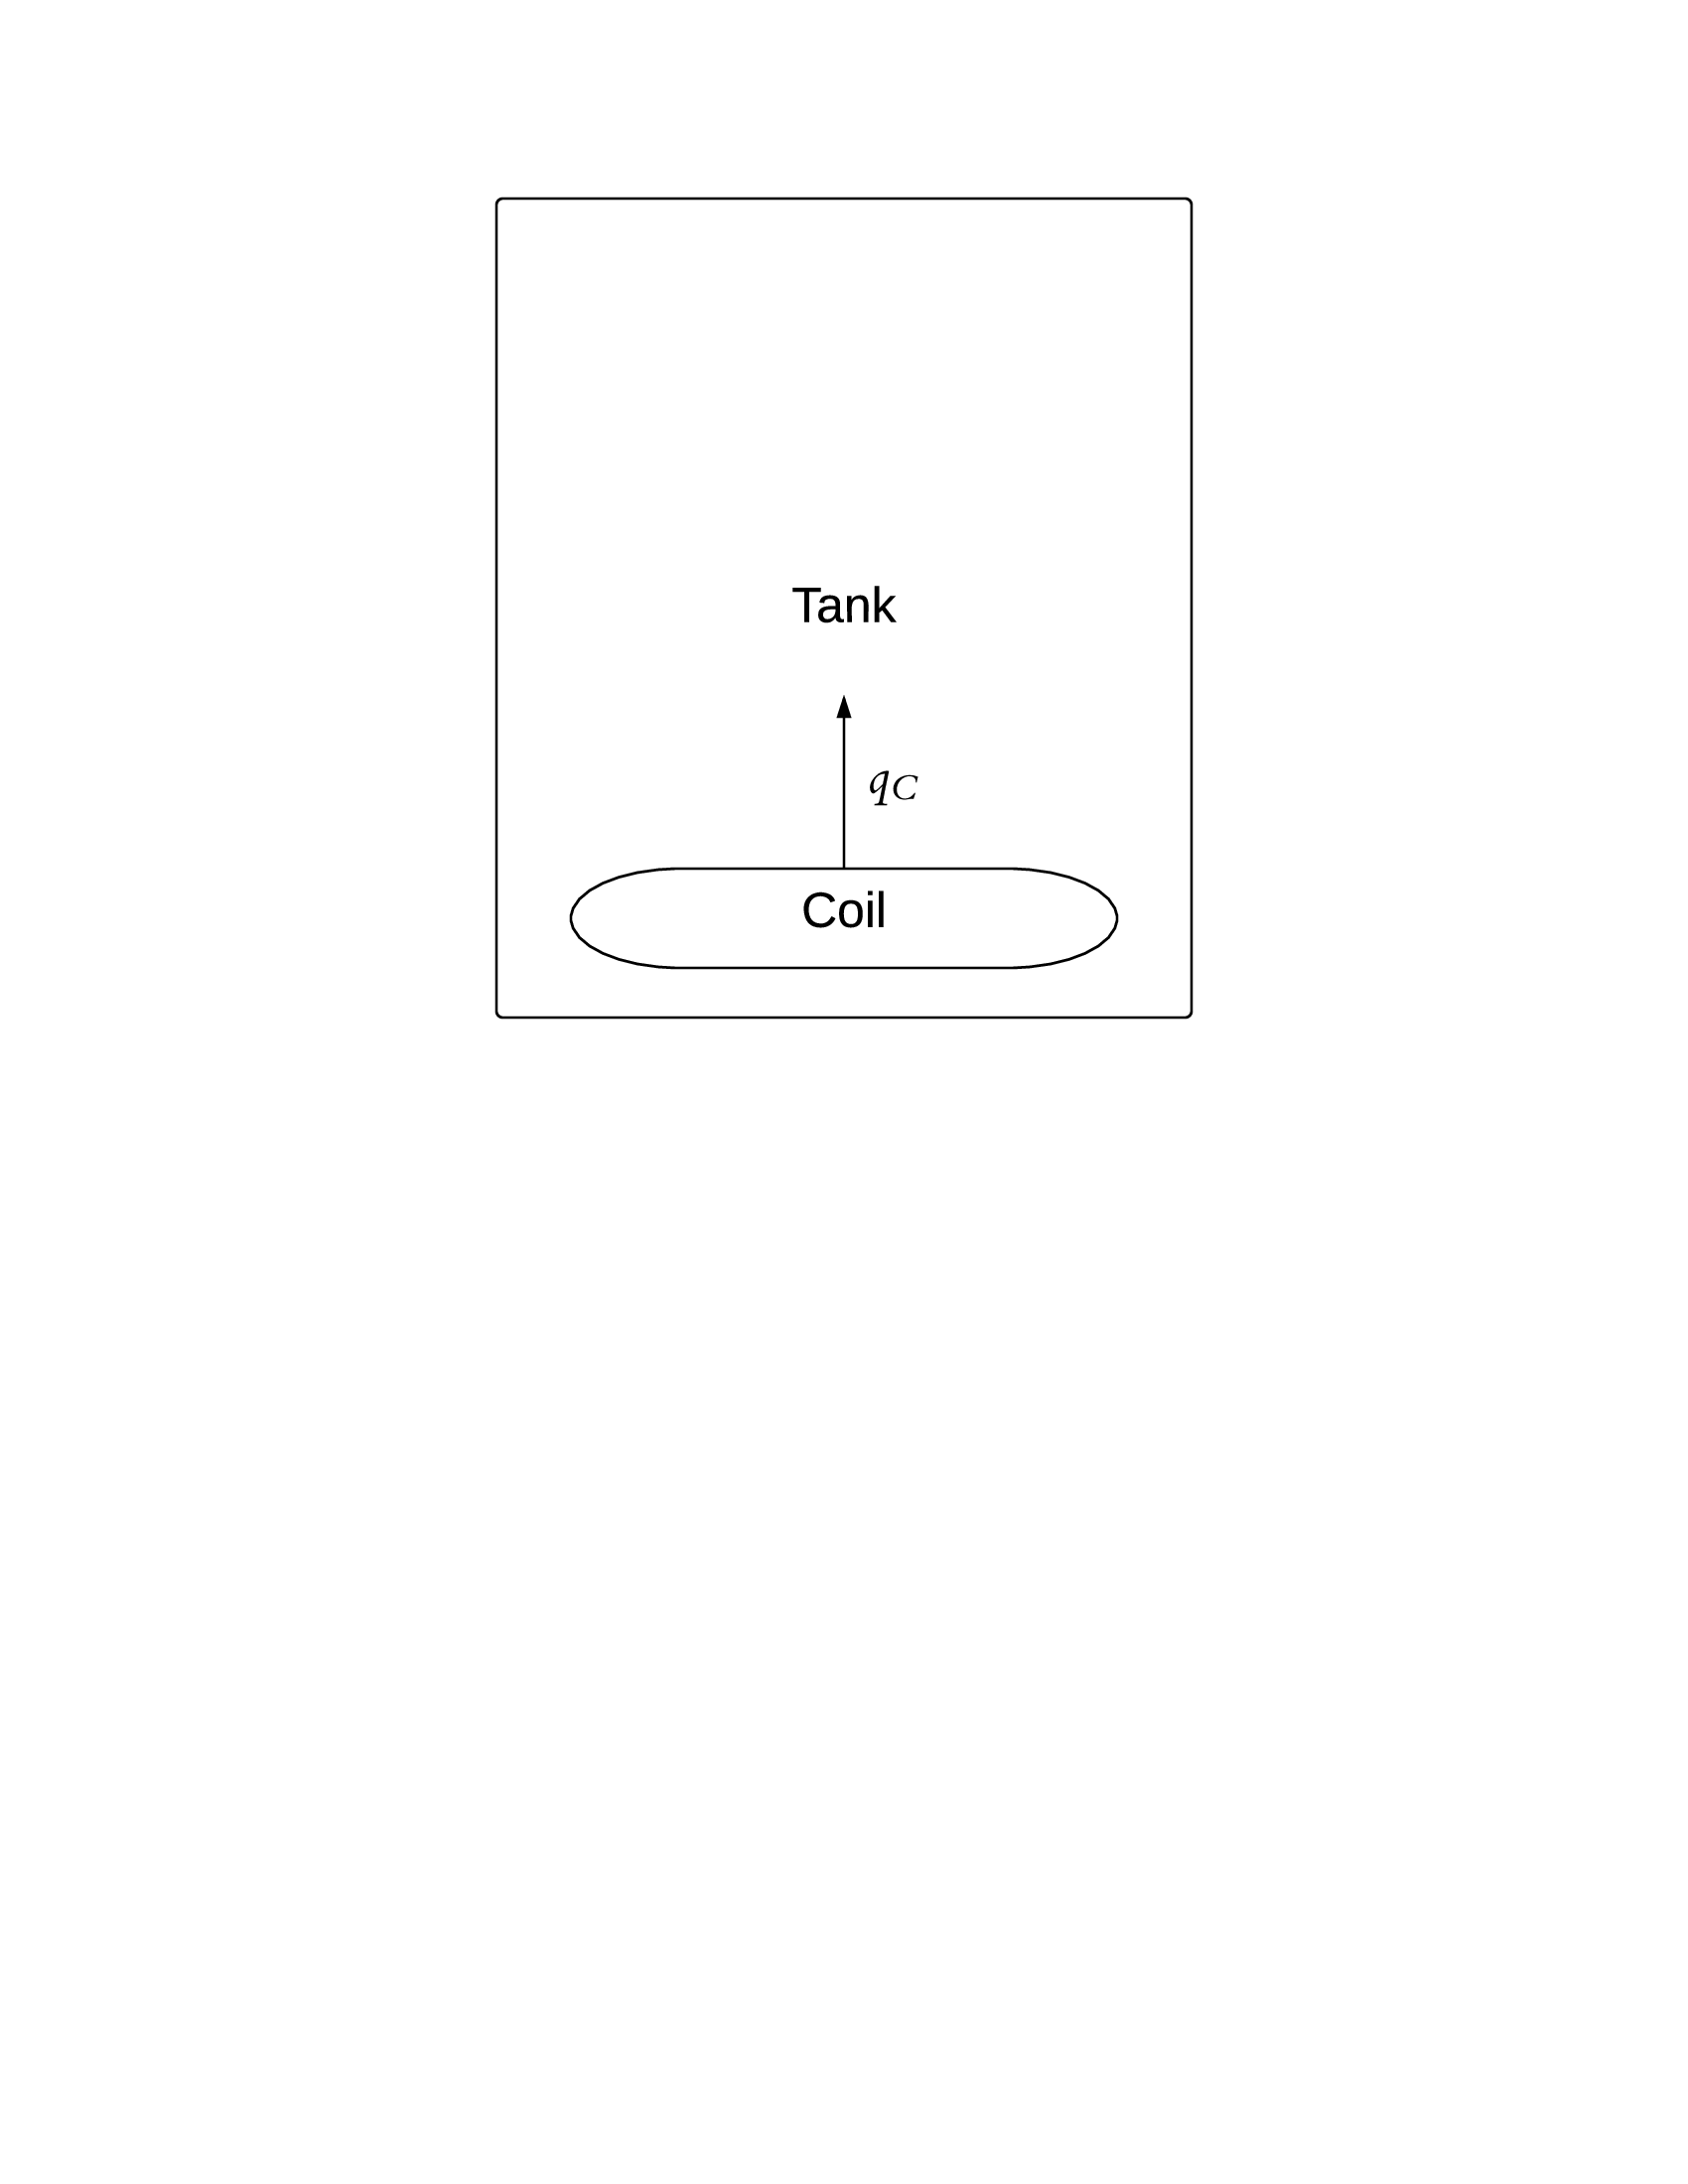
\includegraphics{TankWaterOnly.png}
\caption{Solar water heating tank, with heat flux from coil of $q_{C}$}
\label{Figure:Swhtwhffco}
\end{center}
\end{figure}
\subsubsection{Goal Statements}
\label{Sec:GS}
Given the temperature of the coil, initial temperature of the water, and material properties, the goal statement is
\begin{itemize}
\item[GS1:]predict the temperature of water over time
\end{itemize}
\subsection{Solution Characteristics Specification}
\label{Sec:SCS}
The instance model (ODE) that governs SWHS is presented in . The information to understand the meaning of the instance model and its derivation is also presented, so that the instance model can be verified.
\subsubsection{Assumptions}
\label{Sec:A}
This section simplifies the original problem and helps in developing the theoretical model by filling in the missing information for the physical system. The numbers given in the square brackets refer to the theoretical model [T], general definition [GD], data definition [DD], instance model [IM], or likely change [LC], in which the respective assumption is used.
\subsubsection{Theoretical Models}
\label{Sec:TM}
This section focuses on the general equations and laws that SWHS is based on.
~\newline
\noindent \begin{minipage}{\textwidth}
\begin{tabular}{p{0.2\textwidth} p{0.73\textwidth}}
\toprule \textbf{Refname} & \textbf{T:Cote}
\phantomsection 
\label{T:Cote}
\\ \midrule \\
Label & Conservation of thermal energy
\\ \midrule \\
Equation & $-\nabla{}\cdot{}\mathbf{q}+g=\rho{}C\frac{\partial{}T}{\partial{}t}$
\\ \midrule \\
Description & This equation gives the conservation of energy for time varying heat transfer in a material of specific heat capacity $C$ and density $\rho{}$, where $\mathbf{q}$
\\ \bottomrule \end{tabular}
\end{minipage}\\
\end{document}
